\documentclass[11pt]{article}
\usepackage[margin=1in]{geometry}
\usepackage[T1]{fontenc}
\usepackage{lmodern}
\usepackage{amsmath,amssymb,booktabs,graphicx,microtype}
\usepackage[colorlinks=true,linkcolor=blue,urlcolor=blue,citecolor=blue]{hyperref}
\usepackage{enumitem}
\setlist{nosep}
\newcommand{\OpCount}{28}
\newcommand{\SkipCount}{28}
\newcommand{\ScenarioCount}{108}

\title{Execution phase and token blocking shape low-precision language-model inference}
\author{Dr. Lin Wang\\\small Working paper}
\date{September 11, 2026}
\begin{document}
\maketitle

\begin{abstract}
Weight compression reduces model storage, but its performance benefits depend on
how inference is executed. We examine this dependence on an Apple M4 Pro using
Qwen2.5-1.5B-Instruct in F16, Q8\_0 and Q4\_K\_M formats. In the measured
configuration, F16 achieves the highest mean throughput for 2048-token prompt
processing on both CPU and Metal, whereas Q4\_K\_M achieves the highest mean
throughput for 128-token single-stream generation, exceeding F16 by 2.78$\times$
and 1.93$\times$, respectively. A complementary Q4-only study comprises 72
benchmark invocations across 1.5B and 7B models, two backends, prompt lengths and
token-block limits. Within this study, changing the token-block limit reverses
the observed CPU--Metal ranking for 7B prompt processing. This experiment varies
software blocking, not request concurrency. On the 1.5B model, Q4\_K\_M increases
perplexity from 8.9573 to 9.3102 on a WikiText-2 subset and reduces normalized
HellaSwag accuracy from 61.5\% to 60.0\% on 200 tasks; Q8\_0 yields scores close
to F16. These descriptive quality results do not establish equivalence or a
statistically resolved difference. Reference operators and uncalibrated analytical
scenarios provide complementary tests of representation cost and conditional
hardware benefit. The findings support phase-specific benchmarking with explicit
software blocking controls; they do not establish the benefit of switching formats
within a request or of introducing dedicated hardware.

\end{abstract}

\section{Introduction}
Reducing the precision of neural-network weights changes both their representation
and the operations required to use them. A smaller payload can reduce data transfer,
while unpacking, scaling and implementation-specific scheduling can introduce
additional work. Consequently, storage reduction alone does not specify the
performance of an inference system. The relevant comparison must include the model,
weight format, execution phase and software configuration.

We ask whether the ranking of weight formats is preserved between prompt processing
and autoregressive generation, and whether software token blocking changes the
relative throughput of CPU and GPU execution. The first question is evaluated with
three formats of Qwen2.5-1.5B-Instruct; the second uses Q4\_K\_M variants of 1.5B
and 7B models. These experiments address different comparisons: the format ranking
within a backend and the backend ranking at a fixed format. Neither comparison by
itself determines the optimal microarchitecture.

We denote the number of tokens in a prompt-processing test by $P$, the number of
generated tokens by $D$, the logical token-batch limit by $B_{\mathrm{tok}}$, and
the physical microbatch limit by $U_{\mathrm{tok}}$. These limits govern software
blocking and do not specify the number of independent requests. Separate prompt
and generation tests are not interpreted as generation conditioned on the measured
prompt. Below, $G$ denotes quantization group size and $B$ denotes a byte count;
these quantities are distinct from token-block limits.

The study combines three complementary forms of evidence. Pretrained-model
benchmarks measure phase-specific throughput and descriptive quality differences.
A separate reference implementation exposes the storage and numerical consequences
of an explicitly defined grouped format, including constrained selection on
synthetic networks. Finally, an analytical model states the assumptions under which
additional compute or unpacking throughput could be useful. The custom format is
not the GGUF format used by the pretrained models, and the analytical model is not
calibrated against those measurements. These components therefore do not constitute
an end-to-end validation of a new quantization method or hardware feature.

\paragraph{Experimental scope.}
The host is an Apple M4 Pro with 12 CPU cores, 24 GB unified memory and a 16-core
Apple GPU. The custom CPU implementation is a single-thread reference kernel;
llama.cpp supplies the pretrained-model CPU and Metal execution paths. Dominant
instructions, memory traffic and resource utilization have not been profiled.
The Metal results concern an Apple GPU and do not establish performance on Arm
GPU or NPU products. No measured energy or synthesized area result is used in the
present analysis.

\section{Background and Related Work}
Hardware-aware mixed-precision selection predates this artifact. HAQ explicitly
incorporates hardware feedback into quantization-policy search~\cite{haq}. Our
small exhaustive search is not a replacement for that research contribution: it
uses three synthetic layers, six choices per layer, and an additive measured CPU
cost. The purpose is to make the constraint and evidence chain inspectable.

AWQ couples activation-aware weight quantization with implementation choices for
on-device inference~\cite{awq}. EdgeDecode does not implement AWQ's transformations
and does not reproduce its model-level evaluation. We use a simpler symmetric
format to expose the interaction between scales, group size, packed access, and
runtime. The pretrained-model experiments below compare existing GGUF variants through
llama.cpp; they do not evaluate the custom format against AWQ.

The Roofline framework relates operational intensity to compute and data-transfer
limits~\cite{roofline}. We extend a simplified maximum-stage expression with a
decode-throughput term for illustrative sensitivity analysis. This expression
assumes ideal overlap and is not a fitted predictor of the measured CPU code.
Production-oriented libraries such as KleidiAI are relevant future baselines for
Arm-targeted kernels~\cite{kleidiai}; our scalar implementation should not be
interpreted as their attainable performance.

\section{Representation and Execution}
\subsection{A fully specified grouped format}
Let $W\in\mathbb{R}^{M\times K}$, and let a group contain $G$ consecutive weights
within a row. We pad the reduction dimension to
$K_p=G\lceil K/G\rceil$. For bitwidth $b\in\{4,8\}$ define
$q_{\max}=2^{b-1}-1$. A nonzero group uses scale
$s=\max_j|w_j|/q_{\max}$ and quantized integers
\begin{equation}
q_j=\operatorname{clip}\!\left(\operatorname{rint}(w_j/s),
-q_{\max},q_{\max}\right).
\end{equation}
Zero groups use $s=1$. Rounding follows NumPy's nearest-even rule. The unsigned
stored code is $q_j+q_{\max}$; the highest code is unused. Four-bit codes are
packed low nibble first. Scales use FP32; activations and accumulators also use
FP32. This is an artifact-specific format, not GGUF, AWQ, or a vendor ABI.

The exact weight payload, including scale metadata and padding, is
\begin{equation}
B_W=M K_p b/8+4M\lceil K/G\rceil.
\label{eq:bytes}
\end{equation}
For divisible dimensions, the scale overhead is $32/G$ bits per weight. At
$G=32$, a nominal 4-bit format therefore uses 5 bits per weight, before host object
metadata. Reporting only the nominal precision would omit a material part of the
representation cost.

\subsection{Reference execution paths}
The C operator computes $Y=X\widehat W^T$. Within each output element it decodes
integer codes, accumulates an activation dot product for each group, and applies
the group's scale. It does not expand the entire weight matrix before execution.
The F32 baseline follows the same simple row-dot structure and does not call BLAS.
The compiler is invoked with optimization enabled but without explicit
architecture intrinsics or a fast-math option.

The accompanying Metal reference kernel assigns one output element to each thread
and uses persistent shared buffers. Its call boundary includes command submission,
completion waiting and output copying, while compilation and buffer construction
are excluded. The reference-operator results reported below are CPU measurements.
The pretrained-model Metal measurements use llama.cpp rather than this custom
kernel; they are a separate experiment.

\subsection{Correctness before timing}
Every measured operator is compared with NumPy multiplication using the unpacked
quantized weights. Thus a low-bit error relative to original weights is distinct
from an implementation error relative to the quantized representation. Tests cover
zero groups, non-multiple tails, storage size, invalid inputs, endpoint codes,
quantization error bounds, and composed execution. The quantized native operator is
checked with FP32 tolerances that allow different reduction orders.

\section{Quality-Constrained Configuration Selection}
For layer $\ell$, a configuration $c_\ell$ selects a bitwidth and group size from
$\{4,8\}\times\{32,64,128\}$. Given a development set $D$, we use relative output
MSE as a proxy:
\begin{equation}
Q_D(c)=\frac{\sum_{x\in D}\|f(x)-f_c(x)\|_2^2}
{\max(\sum_{x\in D}\|f(x)\|_2^2,10^{-30})}.
\end{equation}
This is not language-model accuracy. It measures agreement with an untrained
floating-point synthetic network. We evaluate the complete composition for every
candidate rather than adding independent layer errors.

Let $\widehat T_\ell(c_\ell)$ be the median measured CPU time for that layer at
$N=1$. Selection solves the finite problem
\begin{align}
\min_c\quad &\sum_\ell\widehat T_\ell(c_\ell)\\
\text{subject to}\quad &Q_D(c)\leq 0.005,\qquad
\sum_\ell B_{W,\ell}(c_\ell)\leq 0.30 B_{\mathrm{F32}}.
\end{align}
We enumerate all $6^3=216$ possibilities. This provides an exact minimum of this
\emph{finite proxy objective}, not a guarantee of minimum composed runtime.
Allocations, Python dispatch, intermediate copies and nonlinearities can invalidate
the additive timing approximation. Selected networks are consequently timed as
complete native compositions, and tested on separate inputs.

The baselines are uniform Q4/G128, uniform Q8/G64, a quality-only minimum under the
same storage constraint, and a uniformly sampled feasible configuration. The random
control is constrained by quality and maximum storage; it is not exactly
byte-matched. All baselines share generated weights and input splits. An identical
configuration may be selected by multiple rules. Its separately measured times
should be read as repeated observations, not evidence of algorithmic differences.

\section{Architecture Scenarios and Budget Conditions}
\subsection{An explicit hypothetical model}
For a linear operator with $N$ input rows, our scenario model assumes the weight
payload is transferred once and FP32 input/output payload is transferred once:
\begin{equation}
B=B_W+4N(K+M).
\end{equation}
Given bandwidth $\beta$, arithmetic throughput $\phi$ in FLOP/s, decode throughput
$\delta$ in weights/s, and launch cost $L$, the ideal-overlap time is
\begin{equation}
T_{\mathrm{scenario}}=L+\max\left(B/\beta,
2MNK/\phi,MK_p/\delta\right).
\label{eq:time}
\end{equation}
This assumes decoded weights can be reused across the input rows with adequate
buffering. The native kernel does not necessarily realize that reuse. The equation
omits tiling losses, spills, contention, activation conversion and detailed
scheduling. In particular, unpacking and arithmetic may compete for the same
execution resources, violating the assumed overlap. The expression is a conditional
idealized model, not a latency predictor for a measured processor. Here, decoding
weights means unpacking their representation; it is distinct from autoregressive
token generation.

\begin{table}[t]
\centering
\begin{tabular}{lrrrr}
\toprule
Hypothetical profile & GB/s & GFLOP/s & Gweight/s & Launch $\mu$s\\
\midrule
CPU-like &30&100&3&1\\
GPU-like &100&2000&20&20\\
NPU-like &20&4000&4&5\\
\bottomrule
\end{tabular}
\caption{Illustrative inputs, not product specifications and not calibrated to the
measured host. Arithmetic throughput uses two FLOPs per MAC.}
\label{tab:profiles}
\end{table}

We sweep three profiles (Table~\ref{tab:profiles}), $N\in\{1,16,128\}$, two
precisions, two group sizes, and baseline/doubled-compute/doubled-decode
scenarios. This yields \ScenarioCount{} rows. The names denote schematic resource
balances only. The NPU-like profile does not assert compatibility with a real NPU
instruction set or compiler. A separate static contract checker identifies
unsupported precision, activation type, grouping, padding, and format requirements
under an explicitly illustrative backend declaration. It never emits a
compilation-success or cycle-measurement claim.

\subsection{Energy and area are different evidence problems}
The repository evaluates an illustrative dynamic-energy expression,
\begin{equation}
E=B e_{\mathrm{external}}+MNK e_{\mathrm{MAC}}+MK_p e_{\mathrm{decode}}.
\end{equation}
The default coefficients (20 pJ/byte, 0.5 pJ/MAC, 0.2 pJ/decoded weight) are
disclosed assumptions. They are not measured or technology-calibrated.
Leakage, control, complete memory hierarchy, and frequency-dependent power are
absent. Doubling a throughput parameter does not supply a new energy coefficient;
feature-related energy changes are explicitly marked unassessed. In particular,
faster execution is not equated with proportional energy savings.

Rather than inventing an area cost for a decode circuit, we derive its acceptable
budget. If baseline area is $A$, a feature adds $\Delta A$, and measured or modeled
speedup is $S$, performance per area improves only if
\begin{equation}
\frac{S}{1+\Delta A/A}>1\quad\Longleftrightarrow\quad
\Delta A/A<S-1.
\label{eq:area}
\end{equation}
This is a break-even condition under equal frequency and the stated performance
objective. It is not an area estimate. RTL synthesis, technology constraints, and
system integration would be needed to compare an actual circuit with this budget.
The speedup and area must refer to the same system boundary. A local operator
speedup cannot be combined directly with total-chip area: its contribution to
end-to-end speedup must first be established. For a baseline time fraction $f$
accelerated by a factor $s$, with other work unchanged and no added overhead,
$S=[(1-f)+f/s]^{-1}$. These conditions exclude unmeasured conversion and integration
costs.

\section{Pilot Methodology and Results}
\subsection{Measurements and splits}
Operator workloads use $(M,K,N)=(256,512,1),(256,512,16),(1024,1024,1)$ and
$(1024,1024,16)$. Weights are Gaussian with variance scaled by the reduction
size; every 31st input column is multiplied by four to introduce heterogeneity.
Inputs are Gaussian. The four shapes and seven formats produce \OpCount{} CPU
measurements. Each configuration receives two warmups and nine timed repetitions.
Configuration blocks are shuffled with a fixed seed. Inputs remain resident and
hot across repetitions. We report medians and interquartile ranges (IQR), not
confidence intervals. There is no cache flush, affinity control, thermal control,
or DRAM-bandwidth claim.

The network experiment uses three weight seeds (11, 23, 37), with layer shapes
$(192,256)$, $(128,192)$, and $(64,128)$; tanh follows the first two layers. Each network
has 96 development inputs and 256 independently seeded test inputs. Test outputs
are not consulted during selection. The three seeds are a small pilot, not a
population-level statistical validation.

\begin{figure}[t]
\centering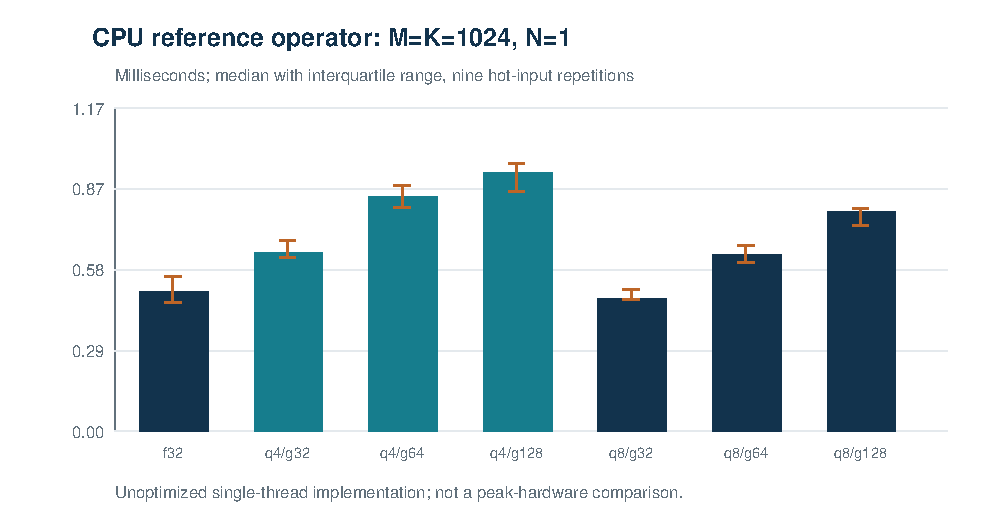
\includegraphics[width=0.95\linewidth]{figures/operator.pdf}
\caption{Actual CPU reference measurements. Error bars denote the IQR of nine
hot-input repetitions. The implementation is intentionally simple and is not an
optimized-library baseline.}
\label{fig:operator}
\end{figure}

\begin{table}[t]
\centering\small\begin{tabular}{lrrrr}
\toprule
Format & KiB & Median ms & IQR ms & Rel. MSE \\
\midrule
f32 & 4096 & 0.506 & 0.093 & 2.90e-13 \\
q4\_g32 & 640 & 0.647 & 0.064 & 1.80e-02 \\
q4\_g64 & 576 & 0.846 & 0.080 & 2.97e-02 \\
q4\_g128 & 544 & 0.932 & 0.104 & 4.27e-02 \\
q8\_g32 & 1152 & 0.480 & 0.037 & 5.29e-05 \\
q8\_g64 & 1088 & 0.639 & 0.061 & 7.98e-05 \\
q8\_g128 & 1056 & 0.795 & 0.062 & 1.19e-04 \\
\bottomrule
\end{tabular}

\caption{Measured example: $M=K=1024$, $N=1$. Payload includes scales and padding.
Relative MSE compares outputs against original F32 weights.}
\label{tab:operator}
\end{table}

\subsection{Compression does not establish acceleration}
Table~\ref{tab:operator} and Figure~\ref{fig:operator} show a concrete counterexample
to treating nominal precision as a speed guarantee. Q4/G32 stores 640 KiB versus
4096 KiB for F32, a 6.4-fold payload reduction. Its measured median latency in this
pilot is nevertheless higher than the F32 reference. Within Q4, changing group size
changes both reconstruction error and runtime. These differences cannot be
attributed solely to external-memory traffic: data may reside in cache, decoding
and accumulation interact, and compiler-generated instructions were not profiled.

The comparison does not show that optimized four-bit execution is intrinsically
slow. It shows that a compression result and a claim about a concrete execution
path are separate propositions. Similarly, subtracting a streaming-copy benchmark
from this operator would not isolate a pure decode cost because access patterns
and overlap would differ.

\subsection{The quality constraint rejects mixed bitwidths}
All three synthetic networks have exactly 27 feasible configurations at the chosen
quality and storage constraints. Every feasible configuration uses eight-bit
weights in all three layers; the 27 possibilities arise from group choices.
Consequently, no result in this pilot demonstrates a mixed-bitwidth advantage.
The hardware-aware rule and the quality-only rule both select Q8/G32 in each layer
for each seed. Timing differences between those labels are repeated measurements
of identical computations, not gains attributable to selection policy.

\begin{table}[t]
\centering\small\begin{tabular}{rlrrr}
\toprule
Seed & Selection & Dev. MSE & Test MSE & CPU ms \\
\midrule
11 & Q4/G128 & 0.14275 & 0.14804 & 0.156 \\
11 & Q8/G64 & 0.00031 & 0.00033 & 0.133 \\
11 & HW-aware & 0.00019 & 0.00022 & 0.125 \\
23 & Q4/G128 & 0.14716 & 0.15306 & 0.152 \\
23 & Q8/G64 & 0.00032 & 0.00033 & 0.135 \\
23 & HW-aware & 0.00022 & 0.00022 & 0.130 \\
37 & Q4/G128 & 0.15434 & 0.15551 & 0.151 \\
37 & Q8/G64 & 0.00035 & 0.00033 & 0.144 \\
37 & HW-aware & 0.00023 & 0.00022 & 0.125 \\
\bottomrule
\end{tabular}

\caption{Development/test relative MSE and independently measured composed CPU
latency. HW-aware selects Q8/G32 in every layer for all three seeds. The Q4 baseline
violates the quality constraint and must not be treated as an eligible winner.}
\label{tab:search}
\end{table}

\begin{figure}[t]
\centering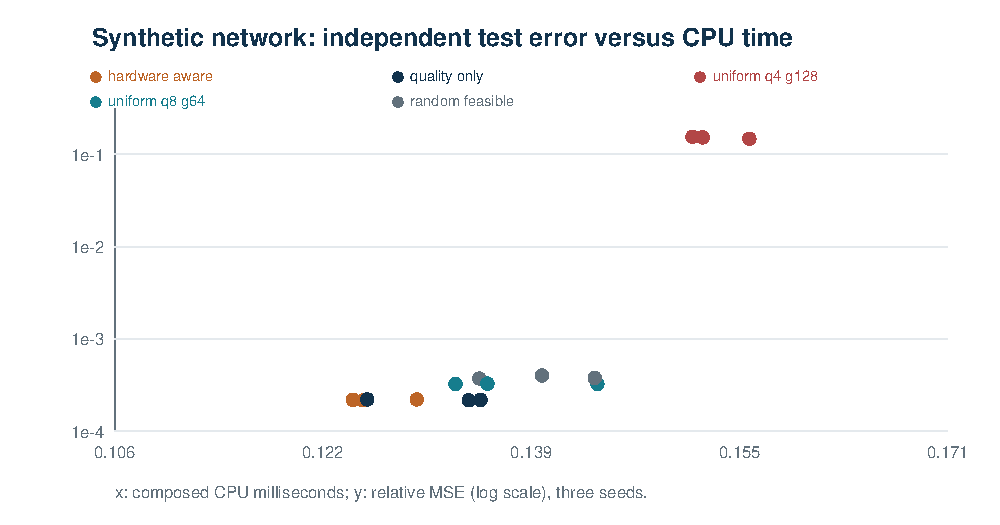
\includegraphics[width=0.95\linewidth]{figures/search.pdf}
\caption{Synthetic-network held-out error and composed timing. Three seeds and
separately measured repeated configurations expose uncertainty rather than
establishing a robust ranking between close timings.}
\label{fig:search}
\end{figure}

The additive cost proxy is not assumed to predict composed latency exactly. In
particular, native composition creates runner objects, copies intermediate outputs,
and applies tanh; these costs are absent from the per-layer lookup. The report
retains both predicted and actual times so that disagreements remain visible.
No calibration-error target or speedup claim is inferred from this small sample.
A larger, optimized experiment would need held-out timing validation and an
appropriate uncertainty model before using this cost function for architecture
recommendations.

\subsection{Hypothetical feature evaluation}
Figure~\ref{fig:architecture} illustrates how doubled decode throughput can lose
value when memory transfer, computation, or launch dominates. This behavior follows
from Equation~\ref{eq:time} and the disclosed parameters; it is not additional
hardware evidence. A feature with $S=1$ has no positive extra-area budget under
Equation~\ref{eq:area}. A feature with higher scenario speedup creates a conditional
budget, but the budget becomes actionable only after model calibration and area
estimation. No general recommendation to build a decoder follows from this pilot.

\begin{figure}[t]
\centering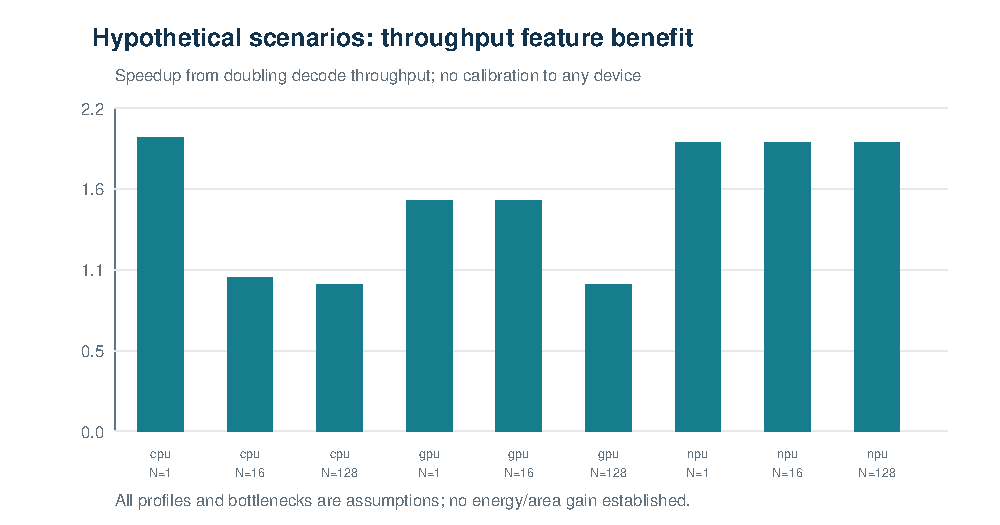
\includegraphics[width=0.95\linewidth]{figures/architecture.pdf}
\caption{Hypothetical feature sensitivity for Q4/G32, $M=K=1024$. These points are uncalibrated scenarios, not measured execution.}
\label{fig:architecture}
\end{figure}

\section{Pretrained-model experiments}
\subsection{Protocol and provenance}
We pin llama.cpp source commit \texttt{451b89bae0c4} and Qwen's official
Qwen2.5-1.5B-Instruct-GGUF repository revision \texttt{91cad51170dc}.
The full revisions and SHA-256 hashes for the
source archive, three model files and two datasets appear in the machine-readable
configuration and manifest. Model weights and datasets are not redistributed.

We use separate CPU-only and Metal-enabled llama.cpp builds with BLAS disabled.
CPU tests use eight threads and zero GPU layers; Metal tests request all layers
on the accelerator. The three-format experiment measures prompt processing at
$P\in\{128,2048\}$ and single-stream generation at $D=128$, with
$B_{\mathrm{tok}}=2048$ and $U_{\mathrm{tok}}=512$. Each of its 18 records contains
seven internal llama-bench timing repetitions. Model--backend jobs are ordered by
a fixed shuffle. The reported throughput is the arithmetic mean of the recorded
rates, not an application-level time-to-first-token or request-latency measure.

Quality is evaluated separately for the same three 1.5B variants: perplexity on
32 context-512 chunks from the WikiText-2 raw test file and normalized accuracy on
200 HellaSwag validation tasks with seed 1234. Quality is not evaluated for the 7B
blocking study. The retained configuration and logs identify the input files,
commands and evaluation subsets.

\subsection{Token blocking changes the observed backend ranking}
The Q4-only extension contains 72 benchmark invocations and 90 output records.
For 1.5B, prompt lengths are $P\in\{128,512,2048\}$ and both token-block limits
are jointly set to 1, 2, 4, 8 or 16. For 7B, prompt lengths are
$P\in\{128,512,1024\}$ and the limits are jointly set to 1, 2, 4 or 8.
Both backends are evaluated, with three timing repetitions per record.

For each model, backend and block setting, an additional invocation specifies
\texttt{-p 128 -n 128}. The pinned benchmark emits separate prompt-only and
generation-only records for this invocation. Its generation record has
\texttt{n\_prompt=0} and \texttt{n\_gen=128}; it does not measure generation
following a 128-token prefill. Of the 90 records, 54 arise from the primary
prompt-processing sweep and 36 from the 18 additional invocations. This protocol
neither varies independent-request concurrency nor measures decode at a controlled
nonzero initial KV-cache length.

At $P=1024$, 7B CPU prompt throughput increases from 6.34 token/s at block limit
1 to 56.19 token/s at block limit 8. Corresponding Metal rates are 44.77 and
44.81 token/s. At $P=128$, CPU rates increase from 28.75 to 78.01 token/s, compared
with 47.65 and 48.90 token/s on Metal. Thus, within the tested block range, the
CPU--Metal mean-throughput ranking reverses at both prompt lengths. Because the
logical and physical block limits change together, their individual effects are
not separated. The deliberately small block limits also do not establish peak
attainable performance for either backend.

This finding concerns backend selection at fixed Q4\_K\_M representation. It
does not show how the preferred precision changes with model scale, because the
7B study contains no F16 or Q8 comparison. Differences between model sizes also
include their architectural differences and are not a controlled intervention on
parameter count alone.

\subsection{Performance is phase dependent}
Table~\ref{tab:stage2-performance} and Figure~\ref{fig:stage2-performance} expose
the central result. On CPU, F16 has the highest mean throughput for 2048-token prefill at 516.1 token/s,
while Q4\_K\_M has the highest mean throughput for 128-token generation at
114.0 token/s, 2.78$\times$
F16. Q8\_0 sits between them at 419.7 token/s in prefill and 70.8 token/s in
decode. On Metal, F16 again has the highest mean prefill throughput at 1872.2 token/s, with Q8\_0
and Q4\_K\_M at 1530.4 and 1287.2 token/s respectively. The generation ranking
reverses: Q4\_K\_M reaches 121.3 token/s, 1.93$\times$ F16.

\begin{table}[t]
\centering\small\begin{tabular}{llrrr}
\toprule
Backend & Phase & F16 & Q8\_0 & Q4\_K\_M \\
\midrule
CPU & Prefill & 516.1 & 419.7 & 357.3 \\
CPU & Decode & 41.0 & 70.8 & 114.0 \\
METAL & Prefill & 1872.2 & 1530.4 & 1287.2 \\
METAL & Decode & 62.8 & 98.8 & 121.3 \\
\bottomrule
\end{tabular}

\caption{Measured Qwen2.5-1.5B throughput in token/s. Prefill uses 2048 tokens;
decode uses 128 generated tokens. Values are llama-bench means over seven samples.}
\label{tab:stage2-performance}
\end{table}

\begin{figure}[t]
\centering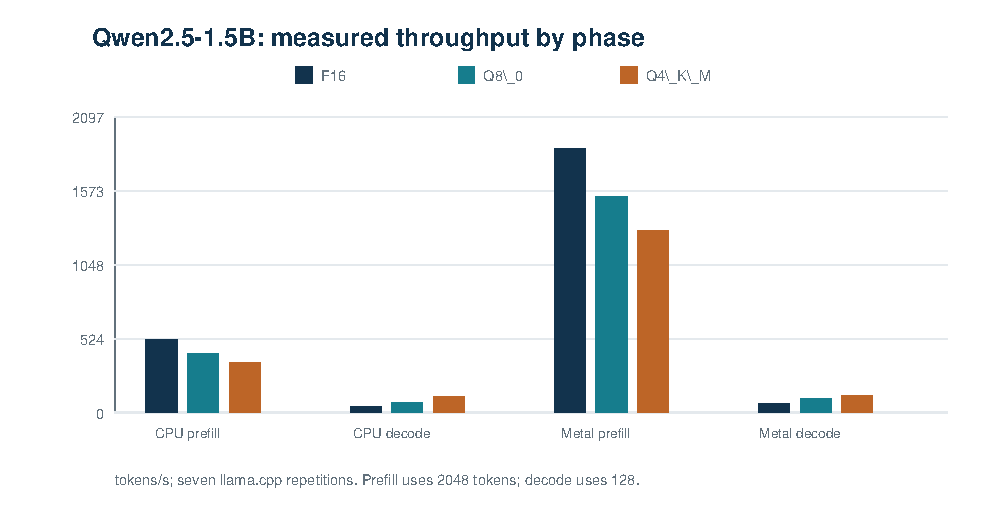
\includegraphics[width=0.97\linewidth]{figures/stage2-performance.pdf}
\caption{The ordering of mean format-specific throughput differs between phases. Apple
Metal measurements are not Arm GPU measurements.}
\label{fig:stage2-performance}
\end{figure}

These measurements show a reversal in the ordering of format-specific mean
throughputs between the two phases. They are consistent with a benefit from lower
weight-transfer volume during single-stream generation, but do not identify a
memory-bandwidth bottleneck or isolate unpacking cost. The formats invoke different
implementation paths, so the comparison evaluates complete format--implementation
pairs rather than nominal bitwidth alone.

The result motivates including execution phase in software selection. It does not
demonstrate that selecting F16 for prefill and Q4 for generation within one request
improves end-to-end performance. Such a policy must account for weight residency,
format conversion or loading, KV-cache compatibility and numerical effects at the
transition. Its request time would include prefill, switching and generation costs,
and its quality would need to be evaluated as a combined system. These quantities
were not measured. No change of hardware substrate follows directly from the
observed format ranking.

\subsection{Quality differences in the 1.5B evaluation}
\begin{table}[t]
\centering\small\begin{tabular}{lrrr}
\toprule
Format & Size (GiB) & WikiText PPL & HellaSwag (\%) \\
\midrule
F16 & 3.32 & 8.9573 & 61.5 \\
Q8\_0 & 1.76 & 8.9524 & 61.5 \\
Q4\_K\_M & 1.04 & 9.3102 & 60.0 \\
\bottomrule
\end{tabular}

\caption{Official GGUF file size and measured quality pilots. HellaSwag uses 200
fixed-seed tasks. Scores are descriptive; no equivalence or paired significance
test is reported.}
\label{tab:stage2-quality}
\end{table}

Q8\_0 yields perplexity 8.9524 compared with 8.9573 for F16, and both attain
61.5\% normalized HellaSwag accuracy. Q4\_K\_M reduces the GGUF file size from
3.32 to 1.04 GiB, increases perplexity to 9.3102 (a 3.94\% relative increase), and
attains 60.0\% HellaSwag accuracy (a 1.5-percentage-point decrease). File size is
not a measurement of peak resident memory or total runtime memory demand.

These results describe the evaluated subsets. Close scores do not establish
quality equivalence, and overlap of marginal confidence intervals is not a test
of the paired accuracy difference. A paired analysis of per-item outcomes would
be needed to quantify that difference; an equivalence claim would additionally
require a prespecified acceptable margin. The present data do not establish
whether the Q4 quality tradeoff is acceptable for a deployment task. They also do
not evaluate a mixed-format prefill--generation policy.

\section{Discussion}
Two observations recur at different experimental levels. The reference operator
shows that reducing storage need not reduce runtime. The pretrained-model study
shows that the ordering of measured formats changes with execution phase, while
the Q4 extension shows sensitivity of backend ranking to token blocking. Together,
these observations justify reporting the complete execution configuration when
comparing low-precision inference. They do not establish a new quantizer, a
universally optimal precision, or a dedicated-hardware advantage.

The analytical scenarios give a conditional interpretation of hardware benefit:
additional throughput matters only when it reduces a limiting term under the
assumed overlap model. That dependence follows from the model construction and
is not independently validated by the benchmark observations. A predictive
architecture study would require measured traffic and instruction behavior,
calibration on a defined workload set, and validation on held-out workloads.

\paragraph{Measurement and inference limits.}
The CPU reference study uses nine hot-input repetitions; the primary llama.cpp
comparison uses seven internal repetitions; the blocking extension uses three.
Python dispatch and copying are part of the reference call boundary, whereas the
reported llama-bench rates use its internal timing boundary. These measurement
scopes are not interchangeable. The blocking extension runs in a fixed order,
which can confound configuration effects with thermal or system drift. No
frequency locking, controlled cache-state protocol, or independent-session
uncertainty estimate is provided. Rankings therefore refer to observed means,
not statistically established performance dominance.

\paragraph{Workload and quality limits.}
The synthetic networks test selection machinery and cannot establish language-model
quality. The pretrained quality evaluation covers one 1.5B model and two small
subsets; the 7B extension measures only Q4 throughput. There is no assessment of
request concurrency, long-context generation at fixed KV occupancy, instruction
following, or the quality of phase-dependent format switching. The synthetic
relative-MSE threshold is an experimental constraint, not a deployment acceptance
criterion.

\paragraph{Hardware scope.}
All pretrained-model results come from one Apple platform. CPU and Metal builds
have distinct execution paths, and the fastest path attainable by each backend
has not been established. A smaller GPU speedup alone does not show low GPU
utilization: bandwidth saturation, synchronization, kernel selection and other
causes remain unresolved. No Arm GPU/NPU execution, calibrated energy comparison,
or synthesized area result is presented. The static NPU contract checker describes
an illustrative interface and does not demonstrate deployment compatibility.

\section{Conclusion}
On the measured M4 Pro configuration, Qwen2.5-1.5B-Instruct has its highest
mean prompt-processing throughput in F16 and its highest mean single-stream
generation throughput in Q4\_K\_M. A separate Q4 study finds that token-block
settings can reverse the observed CPU--Metal ranking for 7B prompt processing.
These results support phase-specific measurement and explicit blocking controls
in low-precision inference comparisons. Establishing a deployment policy or
hardware investment requires further evidence on end-to-end switching costs,
task quality, bottleneck mechanisms and resource consumption.

\section*{Artifact Availability and Disclosure}
The accompanying source repository contains native kernels, Python code, tests,
raw timing samples, every search candidate, source hashes, hypothetical parameter
files, and figure/table generators. Commands are documented in the repository
README. No pretrained weights or external datasets are redistributed. Code and
original documentation use the MIT license. The draft and implementation were
prepared with AI assistance and require human review before external submission.
No institutional affiliation or hardware-vendor endorsement is implied.

\begin{thebibliography}{9}
\bibitem{haq} K. Wang, Z. Liu, Y. Lin, J. Lin, and S. Han.
HAQ: Hardware-Aware Automated Quantization with Mixed Precision.
CVPR, 2019. \url{https://arxiv.org/abs/1811.08886}.
\bibitem{awq} J. Lin et al.
AWQ: Activation-aware Weight Quantization for On-Device LLM Compression and Acceleration.
MLSys, 2024. Original paper version:
\url{https://arxiv.org/abs/2306.00978v4}.
\bibitem{roofline} S. Williams, A. Waterman, and D. Patterson.
Roofline: An Insightful Visual Performance Model for Multicore Architectures.
Communications of the ACM, 52(4):65--76, 2009.
\url{https://doi.org/10.1145/1498765.1498785}.
\bibitem{kleidiai} Arm contributors. KleidiAI: optimized compute routines for Arm CPUs.
Source repository, accessed September 10, 2026.
\url{https://github.com/ARM-software/kleidiai}.
\end{thebibliography}
\end{document}
